\documentclass[b5paper]{book}
\usepackage[utf8]{inputenc}
\usepackage[T1]{fontenc}
\usepackage[english]{babel}
\usepackage[ddmmyy]{datetime}
\usepackage[chapter]{minted}
\usepackage{mdframed}
\usepackage{graphicx}
\usepackage{fancyvrb}
\usepackage{upquote}
\usepackage{xcolor}
\usepackage{amsmath}
\usepackage{subcaption}

\definecolor{folder}{HTML}{325fcf}
\setminted[latex]{frame=lines,linenos,autogobble}
\setminted[bash]{frame=lines,linenos,autogobble}
\newcommand{\ignore}[1]{} % Does nothing. \ignore{$} to trick highlighting.

\newcommand{\latexin}{\mintinline{latex}}
\newcommand{\latexone}{\mint[frame=none,numbers=none]{latex}}

\newcommand{\reflst}[1]{Listing~\ref{lst:#1}}
\newcommand{\reffig}[1]{Figure~\ref{fig:#1}}
\newcommand{\refch}[1]{Chapter~\ref{ch:#1}}
\newcommand{\refsec}[1]{Section~\ref{sec:#1}}
\newcommand{\reftab}[1]{Table~\ref{tab:#1}}

\renewcommand{\dateseparator}{.}

\title{Coding for Non-Coders}
\author{Sigvald Marholm}
\date{\today}

\begin{document}

\maketitle
\tableofcontents

\chapter{Introduction}
Programmers, engineers, scientists and tech-savvy people in general have had the opportunity to learn a bunch of different computer programs and programming languages which makes their everyday work in front of the computer both easier and more efficient. In comparison, less technically oriented people, who lack such a toolbox, often end up using inconvenient tools and therefore end up using inefficient and impractical solutions.

Consider for instance that you have hundreds of photos and you’d like to change the resolution on all of them? Or maybe add a watermark before sharing them? Or change the filename to include the date? Such tasks can be tedious if you don’t know the right tools. However, the file names of all files can be changed using a single command in the Bash command line interface. A script that adds a watermark to every image takes less then 20 lines of code using the Python scripting language. Of course, programming takes time to learn, and it’s not for everybody to become a full time professional programmer. But with the emergence of modern low-threshold scripting languages like Python, why should such handy techniques still be reserved for geeks only?

Another thing which many may benefit from is learning a professional typesetting tool like LaTeX to write documents. Applications, CV’s, reports, slideshows, etc. Because let’s admit it: Most of us aren’t typographists. We don’t know exactly which font to use, which size, which line spacing and which margins to use everywhere to make a document look professional. LaTeX takes care of all that for you, but then you need to tell LaTeX what’s supposed to be a chapter, what’s a new paragraph, and so on. And that’s done by coding. It doesn’t have to be that hard, to start a new chapter with the title “Introduction”, for instance, you simply type 

\latexone{\chapter{Introduction}}
And how do you generate a table of contents in LaTeX? Simple. Because LaTeX know what the chapters are, all you have to do is type:
\latexone{\tableofcontents}
where you want your table of contents.

And as a last example, have you ever had to collaborate with someone to write a document in a normal text processing tool such as Microsoft Word? Then you’ll know it’s a mess. No two people can edit the document at once, despite editing different parts of the file. Documents written in LaTeX, as well as programs written in languages such as Python can be efficiently shared amongs many users using a Version Control System (VCS) such as Git and everyone can work on it simultaneously without stepping on each other’s toes! VCSs like Git also allows you to backtrack the whole history of your documents in case you regret something you once did.

The aim of this little book is to provide the normal guy on the street with at least a small toolbox allowing him or her to work more efficiently. More in a similar manner as professionals. The tools presented are carefully selected because together, they form a minimal toolbox allowing the reader to use a computer in such a rich way. Moreover, they are considered to be more useful, versatile and simple to learn than other alternatives. Admittedly, we will only scratch the surface of all these tools. Just enough to get you started, with pointers of where to look for further information. True, it will not even cover the same depth as most beginner’s books, since it is not the aim of this book to turn you into a programmer. However, it is assumed that the reader, being a generation which has grown up with technology, is capable of finding his/her way around in simple graphical computer programs. Therefore this book will focus on the coding aspects, only providing pointers to which graphical programs may be useful (for instance to make figures in documents).

Finally, each part are self-contained and may be read independently of the other parts (although using Git is kind of meaningless without knowing some other coding).
\chapter{Command Line Interfaces: Handling Files Efficiently}
10 pages
\section{Why bash?}
\section{Which tools you need}

Things to talk about:
\begin{enumerate}
	\item Bash vs. Windows command line, using bash in Windows
	\item Unix file/folder system
	\item Navigating: pwd, cd, ls
	\item Moving stuff: mv, cp, rename
	\item Reading text: cat, more, less
	\item Writing text: nano, vim (because you'll stumble upon it)
	\item Permissions: chmod, chgrp, chown, sudo
	\item Executing programs, \$PATH, and small scripts
	\item Killing programs: ps, kill, killall
	\item .bashrc and ALIAS
	\item Other useful commands: df, ipconfig, iwconfig, etc.
	\item Advanced topics if space: grep, rsync, imagemagick > and >>
\end{enumerate}

Examples to include:
\begin{enumerate}
	\item Change .JPG to .jpg
	\item Append date to filenames
	\item Add execute permissions to scripts and run them
\end{enumerate}
\chapter{Scripting: Automating Small Tasks}
60 pages
\section{Why Python?}
\section{Which tools you need}

\begin{enumerate}
	\item IPython and running scripts
	\item Variables (int,float,char) and operators
	\item Writing to display
	\item Lists and strings
	\item Input arguments
	\item Example: Computing cost of building something
	\item Conditionals
	\item Assignment: Can you afford building something
	\item Loops
	\item Functions
	\item Reading/writing files
	\item Example and Assignment: Todo-list handler
	\item Libraries and namespaces
	\item Example: Plot mathematical functions
	\item Assignment: Plot interest rates
	\item Example: Add watermark to images
	\item Assignment: Make images grayscale
	\item Example: Plotting image histogram
	\item Objects
	\item Further reading and topics
\end{enumerate}
\chapter{Typesetting: Making Beautiful Documents}
40 pages

\section{Why \LaTeX?}
Most people need to write text documents from time to time, be it a CV, an article or a school assignment. Especially if you're writing something you'll use in your profession, you likely want it to \emph{look} professional which just often is not the case when you use what-you-see-is-what-you-get (WYSIWYG) tools like Microsoft Word or LibreOffice Writer. With these kind of tools the author spends time manually tweaking how stuff looks, and most writers just isn't interested enough in typography. In comparison, using \LaTeX{}, the writer focuses solely on the contents of the document. For instance, ``this is a title'', or ``here is a figure''. This is done in terms of coding. But the author does not have to bother about how it looks. \LaTeX{} takes care of that. In fact, this may seem unfamiliar at first, and many novices try to force \LaTeX{} to display stuff in a particular way. My advice: Just don't!

\LaTeX{} certainly comes with a higher learning barrier before you can use it than WYSIWYG tools, but once you get familiar with it, I think you'll find that it's not actually that much slower to write in, and it produces much better results. Also, it always outputs PDF-files which can be read anywhere. You may find a shift in what you spend time on: less time manually placing stuff, more time looking for how to do ``this thing'' with \LaTeX{} on the internet.

There are other alternatives than \LaTeX{} as well, but \LaTeX{} is very well developed and by far the most widespread, at least when it comes to scientific publications and books. We'll also see how to use it for writing slideshow presentations, thus replacing tools such as Microsoft PowerPoint. If there's one professional typesetting tool you want in your toolbox to it's definitely \LaTeX{}.

\section{Which tools you need}
Basically, \LaTeX{} can be written in any plain text editor (like Notepad if you're using Windows) and stored to a file ending with .tex. The .tex file is then \emph{compiled} to generate a .pdf-file using the command line tool \texttt{pdflatex}. We will go through this in a minute. However, most users prefer a more specialized text editor which runs \texttt{pdflatex} for you. Most such editors also supports highlighting, i.e.\ the application of different colors to different parts of the code to make it more readable. Many good editors exist, but we will use Texmaker which works on both Linux, OS X and Windows.

To get \LaTeX{}, you need to install a \LaTeX{}-distribution on your computer. There are several of them, but the code you write is the same for all of them. Proceed according to your operating system to install a \LaTeX-distribution and Texmaker.

\subsection{Linux}
On Linux, TeX Live is the recommended distribution. On Ubuntu, Mint or Debian Linux, you can install TeX Live and Texmaker using the following command:
\begin{minted}{bash}
sudo apt-get install texlive-full texmaker
\end{minted}

\subsection{OS X}
For OS X, MacTeX is the recommended distribution. It is the essentially the same as TeX Live but adds some compatibility to OS X. Download and install MacTeX and Texmaker from the following links:

\begin{verbatim}
http://tug.org/mactex
http://www.xm1math.net/texmaker
\end{verbatim}

\subsection{Windows}
For Windows either TeX Live or MiKTeX can be used, but many find MiKTeX slightly easier to handle. Install MiKTeX and Texmaker from the following links:

\begin{verbatim}
http://www.miktex.org
http://www.xm1math.net/texmaker
\end{verbatim}

\section{Starting a new document}
We will start by going through \reflst{latex:minimal} which is about the minimum code required to start a new document.
\begin{listing}
	\inputminted{latex}{latex/first.tex}
	\caption{A minimal \LaTeX{} document}
	\label{lst:latex:minimal}
\end{listing}
Notice that all \LaTeX{}-\emph{commands} start with a backslash, and may be followed by mandatory \emph{arguments} in curly braces, and optional arguments (\emph{options}) in square brackets like this:

\latexone{\command[option1,option2]{argument1}{argument2}}

The first command in any document is \mintinline{latex}{\documentclass} which tells \LaTeX{} what kind of document it is. Typical arguments are \mintinline{latex}{book} for writing books, \mintinline{latex}{report} for writing reports and \mintinline{latex}{article} for writing, well, articles. The option \mintinline{latex}{[a4paper]} tells \LaTeX{} to produce a document in paper size A4. Other options exists for other paper sizes, font sizes, etc.\ which you can find on the internet whenever you need it.

Next, the functionality of \LaTeX{} can be expanded by including \emph{packages} which provides more features (similar to \emph{modules} in Python or \emph{libraries} in other languages). This is done by the \mintinline{latex}{\usepackage} command, one per package you want to use. To begin with, we need three packages. \mintinline{latex}{babel} specifies the written language and \mintinline{latex}{fontenc} determines the font encoding in the .pdf-file and should usually be T1.

\mintinline{latex}{inputenc} tells \LaTeX{} the character encoding of the .tex files, that is, how each letter is represented by zeros and ones in the input file. The most common letters such as a, b, c, and so on are fairly standard and typically have the same representation in most encoding standards and therefore will work regardless of which encoding you use. Local letters such as æ, ø and å, however, may be represented differently in different encoding standards if they even exist at all. If such special characters aren't printed correctly, the problem is usually the choice of encoding. The encoding selected by the \mintinline{latex}{inputenc} needs to be the same as the ones the editor saves the files in, and it needs to be able to represent all characters in your language (or other characters you may need). Luckily, great effort have been done to make a unified character encoding that just works in all cases; UTF-8. I strongly recommend to just always use UTF-8 like in the above example to avoid any problems, but take care to save the files using UTF-8 encoding. Many text editors (e.g.\ Notepad) by default use other standards such as ISO-8859-1. We'll show how to do this in Texmaker in a second.

The commands \latexin{\title}, \latexin{\author} and \latexin{\date} is used to specify the title and author of the document, along with the date is was written/published.

The next new thing we'll encounter is an \emph{environment}. An environment starts with a \latexin{\begin} and ends with an \latexin{\end}, and affects anything in between. The \latexin{document} environment is where you write what actually goes into the document. Everything before it, is called the \emph{preamble} and is not actually printed to the document. Here we only have one thing inside the document, a title page which is auto-generated by the \latexin{\maketitle} command based on the information we provided in the preamble.

\section{Compiling}
The next step is to compile our minimal example to turn it into a .pdf file. When Texmaker is opened it's toolbar is as depicted in \reffig{latex:texmaker}. To ensure Texmaker saves all files using UTF-8, go to Options$\rightarrow$Configure Texmaker, open the ``Editor'' pane and make sure ``Editor Font Encoding'' is set to UTF-8.
\begin{figure}
	\centering
	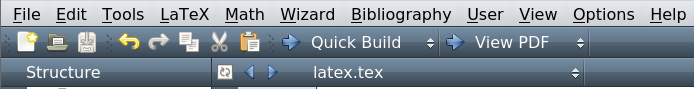
\includegraphics[width=\textwidth]{graphics/texmaker.png}
	\caption{Texmaker toolbar}
	\label{fig:latex:texmaker}
\end{figure}

Create a new file, write the minimal document from \reflst{latex:minimal} in it and save it as \texttt{main.tex} in a new folder. You do want to create a separate folder for each document you write since \LaTeX{} generates lots of other files in this folder upon compilation.

One should be aware that people use different compilation strategies. Some people use the program \texttt{latex} which generates a .dvi file and then converts it to .pdf using a conversion tool, while we will use the program \texttt{pdflatex} which directly generates the .pdf file. Both of these are command line programs but Texmaker can run these commands for us so we don't have to. However, to better grasp what's going on behind the curtains, we will see how it's done both from the command line and from Texmaker. If you haven't read \refch{bash} yet, don't worry. You don't need to be able to run the commands to proceed this chapter.

To compile \texttt{main.tex} using the (Linux, OS X or Windows) command line, navigate to the folder where the file is, and simply run:
\bashone{pdflatex main.tex}
and a file named \bashin{main.pdf} will be created, and you're done.

In Texmaker, we can use the arrow next to ``Quick Build'' drop down menu (see \reffig{latex:texmaker}) to run any of the commands available from the drop down menu. As an example, we can choose ``PDFLaTeX'' and click the arrow, and to view it, we can click the arrow next to ``View PDF''. The ``Quick Build'' option is useful, since it can be configured to run a series of commands in sequence. If you again go to Options$\rightarrow$Configure Texmaker and select the ``Quick Build'' pane you can set Quick Build to ``PdfLaTeX + View PDF''. In the ``Commands'' pane, you can see exactly which commands Texmaker uses when running this programs. Now, when you choose ``Quick Build'' and click the arrow, the document will be compiled and displayed.

Computers are very literal, and care about every tiny mistake you make. If there's a typo somewhere in your code, e.g. a missing letter in a command, the document simply will not compile, but returns an error. The error messages may look cryptic at first, but they do tell what the error is and which line it is on. Try to sort out one error at a time, starting with the top one. Another advice: Compile your document often to avoid a bunch of errors to accumulate.

\section{Document structure}
Now we're going to fill our document with contents, and expand our minimal example to what is shown in \reflst{latex:structure}.
\begin{listing}
	\inputminted{latex}{latex/structure.tex}
	\caption{A \LaTeX{} document with some structure and text}
	\label{lst:latex:structure}
\end{listing}

Documents are split into chapters, which can be split into sections, which again can be split into subsections and further on to subsubsections. The corresponding commands are, intuitively, \latexin{\chapter{...}}, \latexin{\section}, \latexin{\subsection} and \latexin{\subsubsection} and take one argument, which is the name of the chapter, section, subsection or subsubsection.


chapters, sections, subsections, text, comments, tableofcontents, include/input

\section{Assignments}
Change language, change documentclass

\section{References}

\section{Formatting}
Special characters, symbols, emphasize and quotes

\section{Lists}
itemize, enumerate

\section{Figures}
png vs. pdf, references, captions, inkscape

\section{Tables}

\section{Bibliography}

\section{Writing an Application}

\section{Writing a CV using CurVe}

\section{Writing a presentation using Beamer}
\chapter{Version Control: Collaboration and Backtracking}
20 pages
\section{Why Git}
\section{Which tools you need}

\end{document}